\chapter{従来手法を用いた足動作検知実験}
従来手法の枠組みによって構築した足動作検知のBCIについて説明する。
\section{利用したEEGについて}
データとして被験者が8秒間静止と
8秒間足動作を8回繰り返したときに計測されたEEGを用い、
被験者はリラックスできる椅子に着席した状態で前方に配置されたディスプレイの
指示に従って動作を行った(図\ref{fig:asibumi})。
EEGの計測機器としてはg.tec社のg.USBamp\ref{fig:usbamp}を用い、ウェット式の電極を採用した。
ウェット式では頭皮と電極の間に導電性のジェルを注入することでEEGを計測する。
EEGの計測時にはジェルの注入を行いながら、すべての電極に関して電極インピーダンスが\(5k\Omega\)
以下になったことを確認した。
またサンプリング周波数は128Hzとした。
\begin{figure}
    \centering
    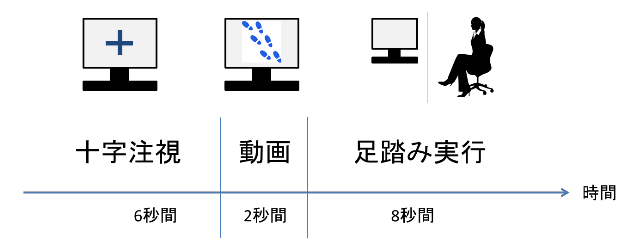
\includegraphics[width=13cm]{images/asibumi.png}
    \caption{EEG計測時のタイムスケジュール}
    \label{fig:asibumi}
\end{figure}
\begin{figure}
    \centering
    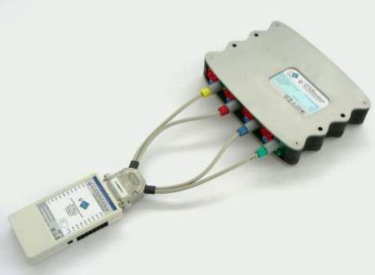
\includegraphics[width=8cm]{images/usbamp.png}
    \caption{g.tec社のg.USBamp}
    \label{fig:usbamp}
\end{figure}

計測に用いた電極の個数は5つであり、Cz、C1、C2、CPz、FCz電極である。
Cz電極は足に関する運動野が脳の頭頂部に存在するため選出し、
スモールラプラシアンフィルタが適用できるように残りの4つを選出した(図\ref{fig:smalllap})。


\section{ERDの解析}
まずEEGの定常成分とERDとは無関係な高周波成分を削除するために
通過帯域を0.3Hzから32Hzとした2次のバタワースバンドパスフィルタを用いた。
その後、空間フィルタとしてスモールラプラシアンフィルタを利用した。
Cz電極で計測したEEGと
Cz電極に対してスモールラプラシアンフィルタを用いた際の
EEGを図\ref{fig:eegsub1}と図\ref{fig:eegsub2}に添付する。
スモールラプラシアンフィルタの定義から、
頭皮上でCz電極に際立った電位分布が獲得されていることが期待できる。
しかし、この処理を行った段階では定量的に
フィルタの是非について議論はできない。

\begin{figure}
    \centering
    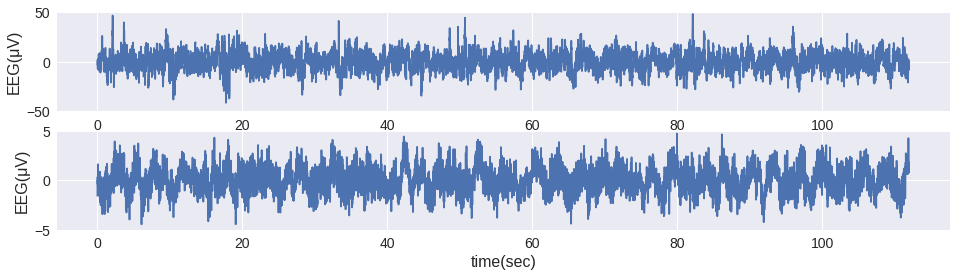
\includegraphics[width=13cm]{images/eeg_sub1.png}
    \caption{被験者1のCz電極のEEG(上)とスモールラプラシアンフィルタを用いたEEG(下)}
    \label{fig:eegsub1}
\end{figure}
\begin{figure}
    \centering
    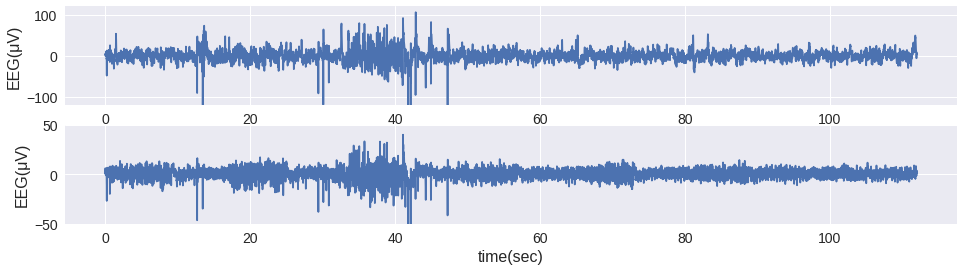
\includegraphics[width=13cm]{images/eeg_sub2.png}
    \caption{被験者2のCz電極のEEG(上)とスモールラプラシアンフィルタを用いたEEG(下)}
    \label{fig:eegsub2}
\end{figure}

% 続いて、PCAとICAによる空間フィルタの設計を試みた。
% それぞれのフィルタから得られる各被験者のEEGの波形を図\ref{fig:bss1}と図\ref{fig:bss2}に示す。
% が\label{section:BSS}にて述べた問題のために、
% 得られた信号のいずれが重要であるかの判断を行うことができなかった。

\subsection{時間周波数解析}
